\title{Implementation of a Kalman Filter}
\author{Joseph Galante}
\documentclass{article}
\usepackage{graphicx}%needed for images
\usepackage{amsmath}%needed for bmatrix and operatorname
\begin{document}

\maketitle

\begin{center}
\Huge 
DRAFT
\normalsize
\end{center}
\vspace{4cm}

Disclaimer

This document is intended to allow a motivated student to understand the basics about how control strategies can be applied for depth control of an AUV.  This document is \emph{not} intended to be a suitable replacement for a classical course in control theory.  Without a thorough understanding of the underlying mathematics and concepts that are glossed over or skipped entirely in this paper, it can be dangerous for a novice to implement these strategies.  When in doubt, seek consultation or supervision from someone experienced.

\newpage

This document works through the implementation of a Kalman filter for the simple problem of determining the position of a box falling under the influence of gravity.  While the problem is very simple, the Kalman filter is an extremely powerful tool and can be applied to other far more complicated problems by going through similar steps.  The first section shows how the falling box can be modeled mathematically.  The TODO STUFF GOES HERE


\section{Problem Statement}


\begin{figure}[h]
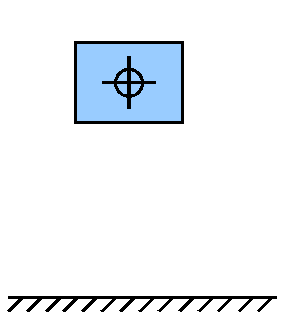
\includegraphics[scale=0.25]{boxPicture.png}
\centering
\caption{The problem: find the position of the box as it falls.}
\label{fig:boxPic}
\end{figure}

Consider a box that initially starts in midair and falls under the influence of gravity.  This document examines the problem of determining the position of the box while it falls.  This might seem like a simple problem.  Perhaps you have seen in a basic physics or calculus course that the position of a box falling with constant acceleration can be derived by simple integration:

\begin{align*}
\ddot{x}(t)&=-\frac{g}{m}\\
\dot{x}(t)&=-\frac{g}{m}t+\dot{x}(0)\\
x(t)&=-\frac{g}{2m}t^2+\dot{x}(0)t+x(0)
\end{align*}






\end{document}